% NeuroCam manual - Network Communication Between Components
% Written by Christopher Thomas.
% Copyright (c) 2021 by Vanderbilt University. This work is released under
% the Creative Commons Attribution-ShareAlike 4.0 International License.

\chapter{Network Communication Between Components}
\label{netcomm}

\section{Overview}

The NeuroCam software consists of several components that interact via UDP 
network messages. A diagram is shown below:

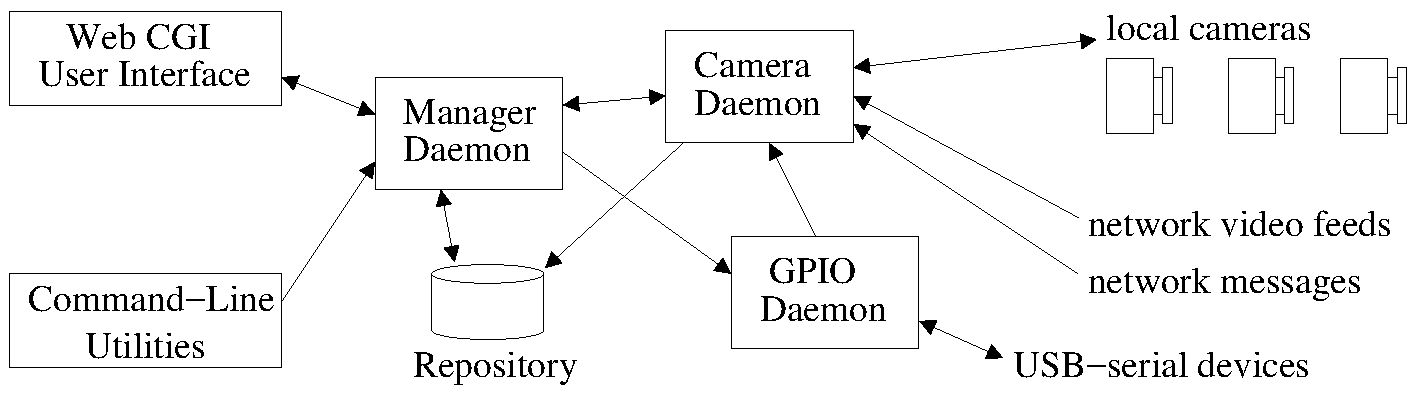
\includegraphics[width=0.9\columnwidth]{figs/dev-netcomm.pdf}

The camera daemon collects local camera video and collects video frames and 
UDP messages from external sources (using the handshaking protocol 
described in Chapter \ref{handshake}).
The GPIO daemon monitors USB-attached serial tty devices, talks to ones
that recognize its handshaking protocol, and reports changes to their state.
The manager daemon coordinates activities at the top level, and a web CGI 
script processes user requests and turns these into commands that are sent 
to the manager daemon.

This architecture was chosen for modularity/compartmentalization. In 
particular, the CGI web interface may be replaced with any other interface
that can talk to the manager daemon over UDP.

% FIXME - Force a page break.
\clearpage
The ports reserved for these communications are defined in the
``\verb+network+'' library file. A summary is below:

\begin{tabular}{ccp{0.7\columnwidth}} \hline
Port & Used By & Purpose \\ \hline
%
7xxx & other &
Default port address range for the network library. Chosen to not conflict
with any other port ranges. \\
\hline
8080 & \verb+fakeunity+ &
Port on which the fake game utility offers its video feed. \\
8090 & (camera) \verb+daemon+ &
Port on which the camera daemon offers the monitoring video feed. \\
8888 & game, \verb+fakeunity+ &
Broadcasts asking for external information sources (videos, UDP messages)
are made to this port. Anything with information to offer should listen 
at this address. \\
\hline
9xxx & (camera) \verb+daemon+ &
Port range reserved for the camera daemon. \\
9998 & (camera) \verb+daemon+ &
Port on which the camera daemon tells itself that it's finished assembling 
a monitoring frame. \\
9999 & (camera) \verb+daemon+ &
Port on which the camera daemon listens for commands. \\
\hline
10xxx & \verb+manager+ &
Port range reserved for the manager daemon. \\
10999 & \verb+manager+ &
Port on which the manager daemon listens for commands/queries. \\
\hline
11xxx & \verb+fakeunity+ &
Port address range reserved for the fake game utility. This is chosen to not 
conflict with any other port ranges. This has to be set to something, because 
the network library can reserve access to ports when used and these will not 
be released until the fake game utility terminates. \\
\hline
12xxx & \verb+cgi+ web script &
Port address range reserved for the CGI script. \\
\hline
13xxx & \verb+mjpeg+ library &
Port range reserved for internal communication by the multithreaded version 
of the video serving function. Multiple instances of that function will 
use overlapping ranges and fight over ports, so the single-threaded version 
should be used when possible. \\
\hline
14000 & \verb+gpio+ &
Port on which the GPIO daemon listens for commands/queries. \\
%
\hline
\end{tabular}

\section{Manager Daemon}

The manager daemon is responsible for starting and stopping the camera daemon,
for ensuring that the GPIO daemon is running, and for performing 
post-processing and other repository manipulations.

The manager daemon listens for UDP packets on port 10999. Commands are
plain text strings.

Multiple commands may be issued in sequence (the manager will accept and
make note of new commands while processing previous commands). Some commands,
like status queries, will be executed immediately even if other tasks are
ongoing; others, like post-processing tasks, will be queued in sequence.

\textbf{NOTE:} Directory paths and filenames are \textbf{not checked}. A
malicious user could abuse this, so it is \textbf{strongly recommended} that 
all such names be script-generated and not based on user input.

Status query command:
\begin{itemize}
\item ``\verb+what is your status reply to port NNNN+''
\end{itemize}

% FIXME - Force a page break.
\clearpage
Status responses:
\begin{itemize}
\item ``\verb+idle+''
\item ``\verb+running cameras+''
%
\item ``\verb+busy (doing what) (progress string)+''

The progress string is optional, and is always in parentheses if present.
The operation specifier (also optional but usually present) is one of the
following:
\begin{itemize}
\item ``\verb+synchronizing timestamps+''
\item ``\verb+compositing+''
\item ``\verb+transcoding+''
\item ``\verb+archiving+''
\item ``\verb+calculating sizes+''
\item ``\verb+removing post-processed files+''
\item ``\verb+removing session folder+''
\item ``\verb+copying session folder+''
\item ``\verb+synchronizing disks+''
\item ``\verb+generating preview+''
\item ``\verb+auto-adjusting cameras+''
\end{itemize}
%
\end{itemize}

Diagnostics commands:
\begin{itemize}
\item ``\verb+debug version to port NNNN+''

The response to this is a version string.

\item ``\verb+debug report to port NNNN+''

The response to this is one or more messages describing the manager's internal
state and the last command processed.
\end{itemize}

Session commands:

\begin{itemize}
\item ``\verb+start cameras repository=(dir) config=(file)+''

Specifying ``\verb+auto+'' for the repository or config file tells the
manager to choose its own values for those parameters. An automatic
repository name will be based on a timestamp.

A copy of the configuration file will be placed in the new session folder.

\item ``\verb+stop cameras+''
\item ``\verb+shut down+''
\end{itemize}

% FIXME - Force a page break.
\clearpage
Monitoring commands (used only while recording):
\begin{itemize}
\item ``\verb+feed (subdir name)+''

The default feed is ``\verb+Monitor+'', which is a stitched-together tiling
of all video feeds. Other feed names just copy one stream's frames directly.
\end{itemize}

Video configuration commands (used only while not recording):
\begin{itemize}
\item ``\verb+snapshot config=(file) outdir=(dir)+''

This acquires frames from all local cameras and all non-local video streams,
saving the results in the ``\verb+auxfiles+'' directory.

\item
``\verb+autocamadjust config=(file) size=(resolution wanted) rate=(fps wanted)+''

This walks through all cameras, adjusting size and exposure settings until
the desired frame rate is obtained. First exposure time is reduced, and if
that fails to produce the desired frame rate size is reduced and the process
repeats. This is very time-consuming.
\end{itemize}

Post-processing commands (used only while not recording):
\begin{itemize}
\item ``\verb+timeshift repository=(dir)+''

This adjusts each video stream's timestamps so that LED flashes are 
synchronized. Only produces valid results if flashes are present.

This creates a modified log file (``\verb+logfile-timed.txt+'') with 
altered timestamps.

\item ``\verb+composite repository=(dir)+''

Assembles a ``Composite'' video feed. This stitches together frames from all
other video feeds, in the same manner as the ``Monitor'' feed, but does so at
higher resolution, with no dropped frames, and with a visible timestamp 
annotation.

This creates a modified log file (``\verb+logfile-composited.txt+'') with
frame events for the ``\verb+Composited+'' video feed inserted.

\item 
``\verb+transcode repository=(dir) stream=(subdir name) output=(file w/o suffix)+''

This assembles frames from one video feed directory into a playable compressed
video file (typically ``\verb+.mp4+'' format).

\textbf{NOTE:} because this performs lossy compression on what was already 
lossy-encoded MJPEG data, the image quality of frames suffers. Compressed 
video files are intended for user preview purposes, not automated processing.

\item ``\verb+archive rootdir=(dir) output=(file without suffix)+''

This creates a ``\verb+.tar+'' archive with the contents of a directory
(typically a session folder). This is intended to allow convenient web 
download of a folder's contents.

\item ``\verb+unprocess repository=(dir)+''

This removes all post-processing files associated with a directory (which
should be a session folder). This includes modified/annotated log files,
compressed video streams, the ``Composite'' video stream's folder, and any
``\verb+.tar+'' archive created of this directory.

\item ``\verb+cancel processing+''

This halts post-processing. The command in progress is killed, remaining
queued commands are purged, and an ``\verb+unprocess+'' command is
automatically queued for execution.
%
\end{itemize}

Repository manipulation commands (used only while not recording):
\begin{itemize}
\item ``\verb+metadata rootdir=(dir)+''

This refreshes metadata for all session folders within a given repository
root directory. This can take quite a while, as updating a changed session 
folder potentially involves checking metadata for millions of files.

\item ``\verb+copy source=(dir) dest=(dir)+''

This duplicates a directory tree (which is intended to be a session folder). 
The original is left intact; for a ``move'' operation, issue a 
``\verb+delete+'' command following this one.

\item ``\verb+delete repository=(dir)+''

This removes a directory tree (which is intended to be a session folder).

\item ``\verb+disksynch+''

This issues a ``\verb+sync+'' command, committing changes to disk. This is
intended to allow safe removal of USB drives, which can take substantial
amounts of time to commit changes.
%
\end{itemize}

\section{Camera Daemon}

\fixme{Content goes here.}

\section{GPIO Daemon}

\fixme{Content goes here.}

Talk about handshaking with GPIO devices over USB-serial.

\section{Web Interface Notes}

\fixme{Content goes here.}

Talk about where scratch files go, what the default directories are,
and the paradigm the CGI script uses.

\fixme{Stopped here.}

%
% This is the end of the file.
